\section{Fortune's algorithm}
In this section we will present an algorithm which computes $\Vor(P)$ in $\mathcal{O}(n \log n)$ time. This is actually optimal, as we can use a Voronoi diagram for sorting:
\begin{thm} \label{thm:voronoicansort}
We can't do better than $\mathcal{O}(n \log n)$.
\end{thm}
\begin{proof}
Let $A = \curly{a_1, a_2, \ldots, a_n} \subset \R$. Now assume we have used an algorithm to compute a Voronoi diagram of the points
\[
    P = \curly{(a_1, 0), (a_2, 0), \ldots, (a_n, 0)}.
\]
We obtain a diagram which looks similar to this:
\[
    
\includegraphics[scale=0.2]{voronoi-sorting}
\]
We assume without loss of generality that the algorithm outputs a DCEL $\Delta$ of $\Vor(P)$. Assume that the $\textsf{edge}$ pointer of every face of $\Delta$ points to the edge to the right of the face, and that the $\textsf{face}$ pointer of every edge of $\Delta$ points to the face to the right. Let $F_i$ be the face in $\Delta$ which contains the point $(0, a_i)$. Let $\ell \in \N$ such that $a_{\ell} < a_i$ for all $i \ne \ell$. Let $b_1 = a_{\ell}$ and if $b_i = a_{j}$ and $i < n$ then define $b_{i+1} = a_k$ where $k$ comes from $F_{j}\textsf{.edge.face} = F_k$. Then $(b_1, b_2, \ldots, b_n)$ is the elements of $A$ in sorted order. This means that we can use the Voronoi diagram to sort, which proves the theorem.
\end{proof}

\todo{The statement of the above theorem is temporary. I originally phrased it like so: ``The optimal worst-case running time for computing $\Vor(P)$ is $\Omega(n \log n)$.'' What is the proper terminology here?} \\

We now present Fortune's algorithm. It is a sweep line algorithm which maintains a horizontal sweep line $\ell \colon y = \ell_y$, and $\ell$ sweeps the plane from top to bottom in order to uncover the structure of the Voronoi diagram. 

For a point $p = (p_x, p_y) \in \R^2$ and a sweep line $\ell \colon y = \ell_y$ the distance between $p$ and $\ell$ is
\[
    \dist(p, \ell) = \abs{p_y - \ell_y}.
\]
Define
\[
    B_i = \makeset{q \in \R^2}{\dist(q, p_i) = \dist(q, \ell)}
\]
for all $i$. If $(p_i)_y > \ell_y$, it turns out we may parametrize $B_i$ by a parabola: Let $p = (p_x, p_y)$ denote $p_i$ and let $q = (x, y) \in B_i$. Since distances are non-negative, it is equivalent to looking at satisfying $\dist(q, p)^2 = \dist(q, \ell)^2$. We have:
\[
    \dist(q, p)^2 = \dist(q, \ell)^2 \iff (p_x - x)^2 + (p_y - y)^2 = (y - \ell_y)^2.
\]
This can be transformed into the equation
\begin{equation}
    2 (p_y - \ell_y) y = x^2 - 2 p_x x + p_x^2 + p_y^2 - \ell_y^2.
\end{equation}
Since $p_y \ne \ell_y$ by assumption, we obtain the parabola:
\begin{equation} \label{eq:parabola}
    y = \frac{1}{2 (p_y - \ell_y)} (x^2 - 2 p_x x + p_x^2 + p_y^2 - \ell_y^2),
\end{equation}
which parametrizes $B_i$ if $(p_i)_y > \ell_y$. Now we look at the situation where $(p_i)_y = \ell_y$. Then
\[
    \dist(q, p)^2 = \dist(q, \ell)^2 \iff (p_x - x)^2 + (p_y - y)^2 = (p_y - y)^2.
\]
Then it must be the case that $p_x = x$, so $B_i$ is a subset of a vertical line, and is a line segment if there is some $B_k$ above $B_i$ and a half-line which starts at $p_i$ otherwise. Finally, if $(p_i)_y < \ell_y$, we let $B_i = \varnothing$. We now for all $i$ define the maps
\[
    \beta_i(x) = \begin{cases}
        \displaystyle \frac{x^2 - 2 (p_i)_x x + (p_i)_x^2 + (p_i)_y^2 - \ell_y^2}{2 ((p_i)_y - \ell_y)} & \text{if } (p_i)_y > \ell_y, \\
        \infty & \text{otherwise.}
    \end{cases}
\]
Let $\textsf{LB}(x)$ denote the map which takes the minimum of each $\beta_i$, i.e.
\[
    \textsf{LB}(x) = \min\curly{\beta_1(x), \beta_2(x), \ldots, \beta_n(x)}.
\]
\begin{defn}[Beach line]
The \emph{beach line for the points $P$ with regards to the sweep line $\ell$} is given by the following subset of $\R^2$:
\[
    G \cup V,
    %\makeset{(x, \textsf{LB}(x)) \in \R^2}{\textsf{LB}(x) < \infty} \cup \makeset{B_i - \curly{(p_i)_x} \times (\textsf{LB}((p_i)_x), \infty)}{(p_i)_y = \ell_y}.
\]
where $G$ is the graph of $\textsf{LB}$ when it is finite
\[
    G = \makeset{(x, \textsf{LB}(x)) \in \R^2}{\textsf{LB}(x) < \infty},
\]
and $V$ is all the vertical parts not hidden behind other parabolas
\[
    V = \makeset{B_i - \curly{(p_i)_x} \times (\textsf{LB}((p_i)_x), \infty)}{i = 1, \ldots, n \text{ where } (p_i)_y = \ell_y}.
\]
\end{defn}
\begin{rmk}
From the definition we see that the beach line consists of parts of parabolas, and vertical line segments or half-lines. For this reason, it is easy to see that the intersection between any vertical line and the beach line has at most one component.
\end{rmk}
\begin{rmk}
For a sweep line $\ell$ which does not intersect any of the points in $P$, it follows from the definition of beach line that the map $\textsf{LB}(x)$ parametrizes the beach line. This was used to make a simple demo visualing the beach line, which can be found in $\boxed{\textsf{demos/beachline}}$.
\end{rmk}
\begin{defn}[Breakpoint]
Every point $q$ on the beach line such that $q \in B_i \cap B_j$ for two different $i, j$ is called a \textit{breakpoint}.
\end{defn}

\begin{figure}[H]
    \centering
    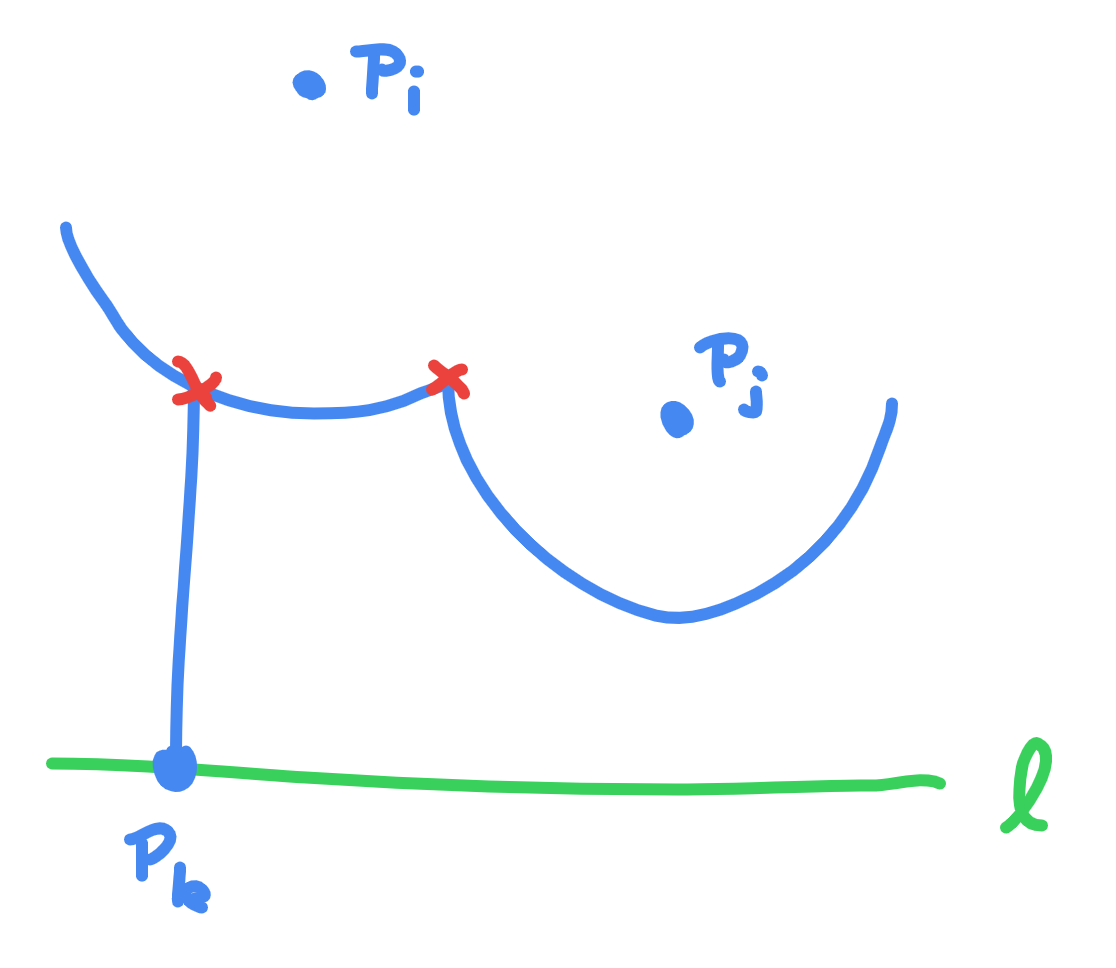
\includegraphics[scale=0.24]{temp-fig-6}
    \caption{The red crosses indicate breakpoints and the blue lines represent the beach line.}
    \label{fig:example-of-breakpoint}
\end{figure}

Now we show that the breakpoints exactly trace out $\VorG(P)$ as the sweep line $\ell$ moves from top to bottom.
\begin{prop}
We have the following:
\begin{enumerate}[{(}i{)}]
\item For every sweep line $\ell$: $y = \ell_y$ each breakpoint lies on $\VorG(P)$.
\item For every point $q$ in $\VorG(P)$ there is a position of the sweep line $\ell$ such that $q$ is a breakpoint.
\end{enumerate}
\end{prop}
\begin{proof}
We prove each statement individually:
\begin{enumerate}[{(}i{):}]
    \item Let $\ell$ be the sweep line, and assume that it has one or more breakpoints. Let $q \in \R^2$ be such a breakpoint. Then $q \in B_i \cap B_j$ for some $i \ne j$, which means that
    \[
        \dist(q, \ell) = \dist(q, p_i) = \dist(q, p_j).
    \]
    The last equality gives us that $q \not\in \mathcal{V}(p_k)$ for all $k$, hence $q \in \VorG(P)$.
    \item Let $q = (q_x, q_y) \in \VorG(P)$. Since $q$ is either an edge or a vertex, Theorem \ref{thm:characterizationofbisectors} gives us that $\partial C_P(q) \cap P$ has at least two elements, so let $p_i, p_j \in \partial C_P(q) \cap P$ be two different elements. We have $\dist(q, p_i) = \dist(q, p_j)$ by definition of $C_P(q)$, and then we may set
    \[
        \ell_y := q_y - \dist(q, p_i),
    \]
    and obtain
    \[
        \dist(q, \ell) = \dist(q, p_i) = \dist(q, p_j).
    \]
    Then $B_i$ and $B_j$ intersect at $q$, and $q$ is on the beach line since there is no $B_k$ with a point $p_k$ closer to $q$ than $p_i$ and $p_j$, by definition of $C_P(q)$.
\end{enumerate}
\end{proof}
As the sweep line $\ell$ sweeps the plane from top to bottom, the combinatorial structure of the beach line changes. We'll categorize these changes into \emph{events}.

First we will consider when new arcs appear on the beach line. As $\ell$ sweeps down and hits a point, a vertical segment is added to the beach line, and then as $\ell$ continues to move, the vertical line spreads out into a new parabolic arc, as seen in this figure:
\[
    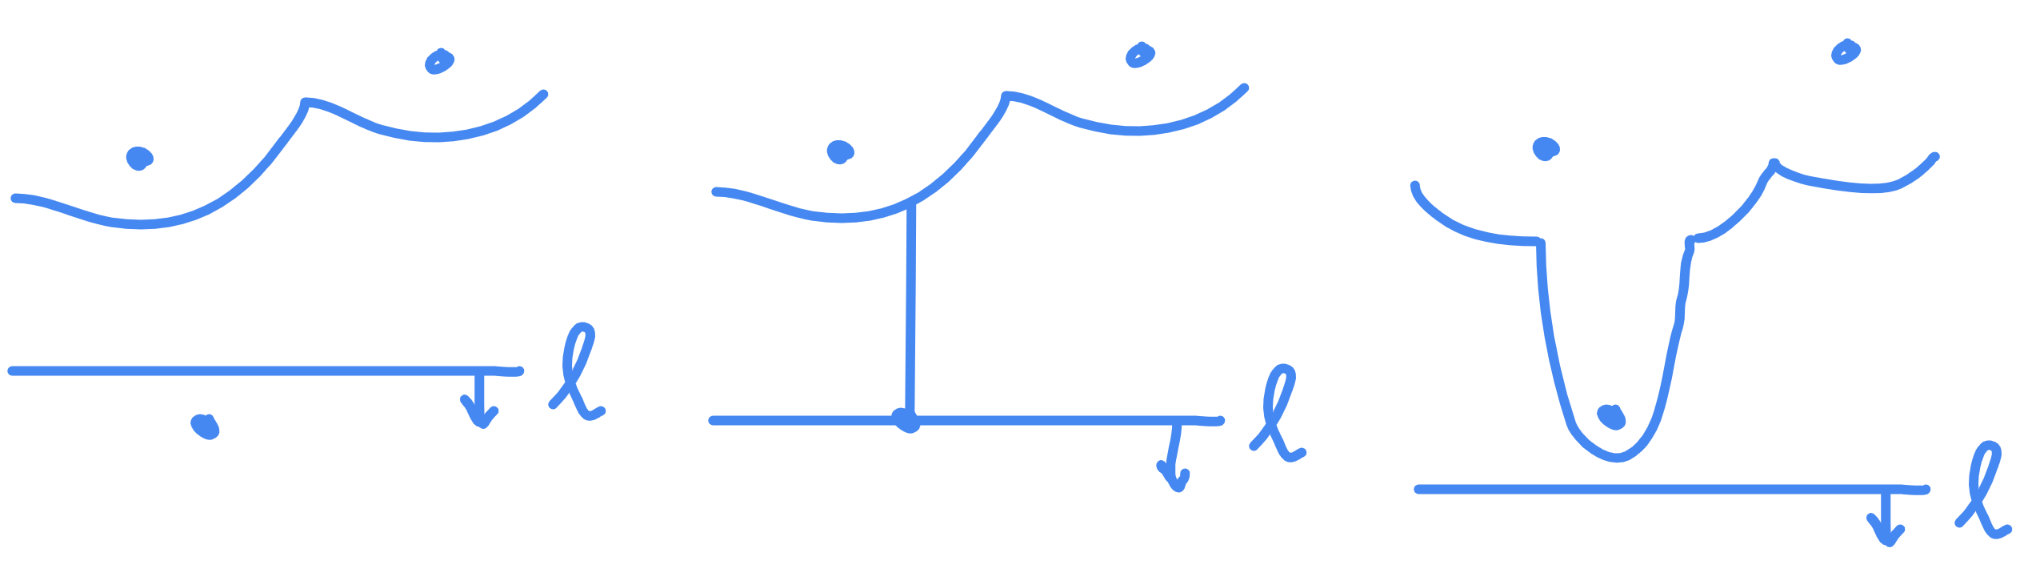
\includegraphics[scale=0.25]{temp-fig-7}
\]
\begin{defn}[Site event]
When $\ell$ encounters a point $p_i \in P$, that is when $\ell_y = (p_i)_y$, we say that we encounter a \emph{site event}.
\end{defn}

\begin{lem} \label{highschoollemma}
If $(p_i)_y = (p_j)_y$ then the parabolas $\beta_i$ and $\beta_j$ intersect in exactly one point. If $(p_i)_y \ne (q_i)_y$ then $\beta_i$ and $\beta_j$ intersect in 2 different points.
\end{lem}
\begin{proof}
Let $p = (p_x, p_y)$ denote $p_i$ and $q = (q_x, q_y)$ denote $p_j$. If $p_y = q_y$ then
\begin{equation}
    \beta_i(x) - \beta_j(x) = \para{\frac{p_x - q_x}{\ell_y - p_y}}x + \frac{q_x^2 + q_y^2 - p_x^2 - p_y^2}{2 (\ell_y - p_y)}
\end{equation}
is a line with non-zero slope since $p_y \ne \ell_y$ and $p_x \ne q_x$, because if $p_x = q_x$ then it would be the case that $p_i = p_j$. Such a line intersects the $x$-axis exactly once.

If $p_y \ne q_y$ then $\beta_i(x) - \beta_j(x)$ is a second degree polynomial with discriminant
\begin{equation}
    D = \frac{(p_x - q_x)^2 + (p_y - q_y)^2}{(p_y - \ell_y)(q_y - \ell_y)}.
\end{equation}
Since $p_y, q_y > \ell_y$ the denominator is strictly positive, and since $p_i \ne p_j$ the numerator is also strictly positive, so $D > 0$. This means that $\beta_i$ and $\beta_j$ intersect in two different points.
\end{proof}

\begin{lem}
The only way in which a new arc can appear on the beach line is through a site event.
\end{lem}
\begin{proof}
Assume for the sake of a contradiction that a new arc appears on the beach line but $\ell_y \ne p_i$ for all $i$. Let $\beta_j$ denote the parabola which contains the new arc, associated to the point $p_j \in P$, which appears on the beach line. We have that $\beta_j$ is a full parabola since $\ell_y \ne p_j$. Now, we look at the two cases in which $\beta_j$ can appear as a new arc on the beach line.

The first possibility is that $\beta_j$ breaks through the middle of an another arc which is a part of the parabola $\beta_i$. For this to happen, there is a time at which $\beta_i$ and $\beta_j$ either coincide, or they are tangent which means they intersect in exactly one point which is on the beach line. They cannot coincide, since $p_i \ne p_j$, so they must intersect in exactly one point. If $(p_i)_y \ne (p_j)_y$ then Lemma \ref{highschoollemma} gives us our contradiction. Otherwise, we have $(p_i)_y = (p_j)_y$. In this case $\beta_i$ and $\beta_j$ have the same shape and the same $y$-coordinate of their inflection points, but their intersections with the $y$-axis differ. Let $q$ be the intersection point of $\beta_i$ and $\beta_j$. Since it is on the beach line, we have $\dist(q, \ell) = \dist(q, p_i) = \dist(q, p_j)$. \todo{Maybe find a contradiction which says that $q$ cannot be on the beach line?}

The second possibility is that $\beta_j$ appears in between two arcs. Let these arcs be part of parabolas $\beta_i$ and $\beta_k$. Let $q$ be the intersection point between $\beta_i, \beta_j$ and $\beta_k$, and we assume that the arc on the beach line from $\beta_i$ is to the left of $q$, and the arc from $\beta_k$ is to the right of $q$, as in this figure:
\[
    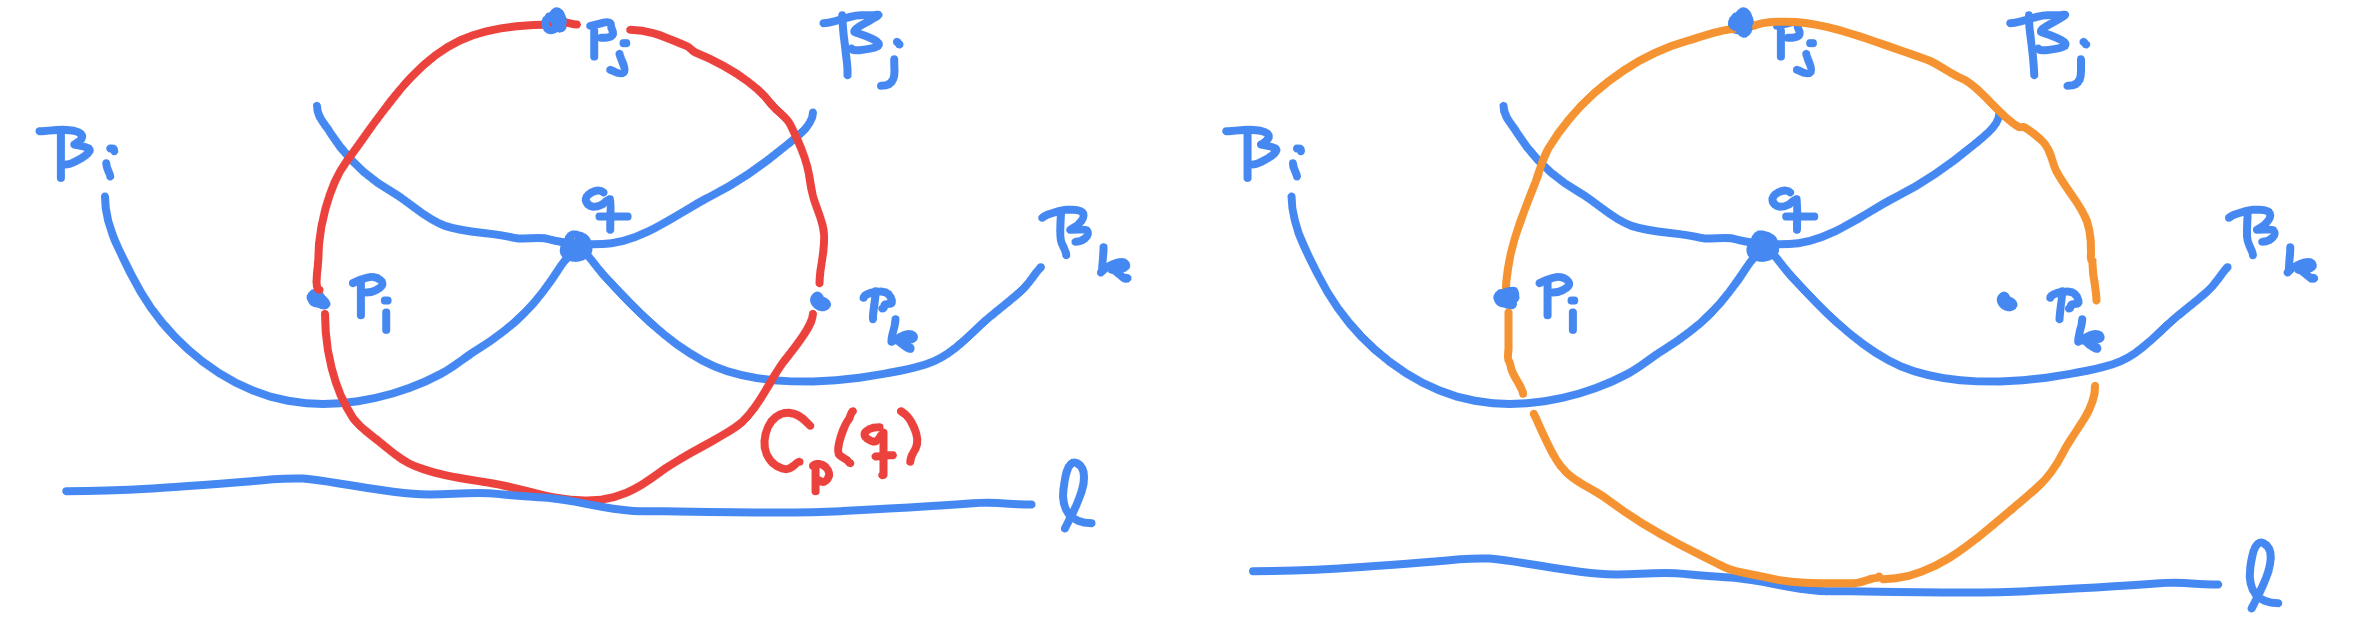
\includegraphics[scale=0.25]{temp-fig-8}
\]
Now let $C$ denote the circle $C_P(q)$. This has $p_i, p_j, p_k$ on its boundary, and it is tangent to $\ell$. The cyclic order on $C$, starting at the point of tangency with $\ell$ and going clockwise is $p_i, p_j, p_k$. Now, we imagine moving $\ell$ downward while keeping $C$ tangent to $\ell$ and $p_j$. Let $q'$ be the new center of $C$. Then either $p_i$ or $p_k$ will be contained in the interior of $C$, which means that there exists a small neighbourhood $U$ of $q'$ where $\dist(p_i, \ell)$ or $\dist(p_k, \ell)$ is less than $\dist(p_j, \ell)$, meaning that points from $\beta_i$ which are in $U$ cannot be on the beach line, contradicting that $q$ is on the beach line. \todo{Make more rigorous?}
\end{proof}
\todo{I do not like the above proof! Maybe some of the literature the CompGeo book references has better proofs.}

%GeoGebra demo of two points and their beach line
%\[
%    \boxed{\text{\url{https://www.geogebra.org/calculator/zreutrt6}}}
%\]